\section{Empirical analysis}
\label{sec:experiment}
%-----------------------------------------------------------
\subsection{Datasets description}

Each of the considered progress prediction methods evaluates on a different dataset: \textsl{RSDNet} on \textsl{Cholec80} \cite{twinanda2016}, \textsl{ProgressNet} on \textsl{UCF101-24} \cite{soomro2012}, and \textsl{UTE} on \textsl{Breakfast} \cite{kuehne2014, kuehne2016}. 
To analyze these methods, we use all 3 datasets for all methods. 

\smallskip\noindent\textbf{\textsl{Cholec80} \cite{twinanda2016}}: Consists of 80 videos of endoscopic cholecystectomy surgery.  
Note that \cite{twinanda2019} uses an extended version of this dataset, \textsl{Cholec120}, containing 40 additional surgery videos. 
However, \textsl{Cholec120} is not publicly available, so we used \textsl{Cholec80} to report our results. 
We randomly create four folds of the data, and follow the same train\slash test dataset split sizes as in \cite{twinanda2019}. 
This dataset has limited visual variability both across training and test splits.
Moreover, the presence of different medical tools in the frames informs of the different surgery phases, which could aid the progress prediction task.

\smallskip\noindent\textbf{\textsl{UCF101-24} \cite{soomro2012}:} Consists of a subset of \textsl{UCF101} containing 24 activities, each provided with a spatio-temporal action tube annotation.\footnote{Following \cite{becattini2017} we use the revised annotations available at \url{https://github.com/gurkirt/corrected-UCF101-Annots}} 
Becattini \etal \cite{becattini2017} split the dataset into 2 categories: \textsl{telic} and \textsl{atelic} activities.
\textsl{Telic} activities are those with a clear endpoint, such as `cliff diving', while \textsl{atelic} activities, such as `walking the dog', do not have a clearly defined endpoint. 
Predicting progress for \textsl{atelic} activities is more difficult than for \textsl{telic} ones.
The original implementation first trains on \textsl{telic} activities, and then fine-tunes on all activities. 
We did not observe a difference when using this training procedure, and instead train all methods on the full dataset.

\smallskip\noindent\textbf{\textsl{Breakfast} \cite{kuehne2014, kuehne2016}:} Contains 10 cooking activities: \eg `making coffee', `baking pancakes', or `making tea', etc., performed by 52 individuals in 18 different kitchens. 
We use the default splits and train each model across all cooking activities. 
Because the tasks are performed by different individuals in different kitchens, the video appearance varies even within the same task, making this dataset extra challenging for progress prediction.

\textsl{UCF101-24} contains training videos of up to 599 frames, while \textsl{Cholec80} and \textsl{Breakfast} contain videos with thousands of frames.
When training on \textsl{full-video} sequences, we could not train the \textsl{ProgressNet} model on the original \textsl{Cholec80} and \textsl{Breakfast} datasets, because of the long videos leading to memory problems.
Thus, for the experiments using \textsl{full-video} sequences, we use a subsampled version of \textsl{Cholec80} from 1 fps to 0.1 fps (the original fps is 25; \cite{twinanda2019} subsamples this down to 1fps); and we subsample \textsl{Breakfast} dataset from 15 fps down to 1 fps. 
For our experiments on \textsl{video-segments} we use the original datasets.

%-----------------------------------------------------
%-----------------------------------------------------
%-----------------------------------------------------
\subsection{Experimental setup}
For the considered progress prediction methods only the code for \textsl{UTE} is published.\footnote{\url{https://github.com/Annusha/unsup_temp_embed}} 
For the other methods, we follow the papers for implementation details and training procedures. 
We train \textsl{RSDNet} in a 2-step procedure following \cite{twinanda2019}, however for training the LSTM blocks we found that using the Adam optimizer with a learning rate of $10^{-4}$ and no weight decay, for $30$k iterations works best. 
For \textsl{ProgressNet} not all training details are mentioned in the paper, so we use Adam with a learning rate of $10^{-4}$ for $50$k iterations, and we keep the VGG-16 backbone frozen during training. 
For all experiments we report the MAE (Mean Absolute Error) in percentages.
% We will release our code.
%-----------------------------------------------------
%-----------------------------------------------------
%-----------------------------------------------------
\subsection{\textbf{\emph{(i) On what information do progress prediction methods base their predictions?}}}
\noindent\textbf{(i.1) Progress predictions on \textsl{full-videos}.}
Here we want to test what information the learning-based models use to predict progress when trained on \textsl{full-videos}.
% Here we want to test what information are the learning-based models using when trained on \textsl{full-videos} to predict activity progress.
For this we evaluate all learning methods when using \textsl{full-video} data as input: \ie either frames or frame embeddings.
We compare this with using \textsl{random-noise} as input. 
If the models learn to extract useful appearance information, their MAE scores should be considerably higher than when inputting \textsl{random-noise}.
Additionally, we compare the learning-based methods with the naive baselines: \textsl{static-0.5}, \textsl{random}, and \textsl{average-index}.

\begin{figure}
\begin{center}
   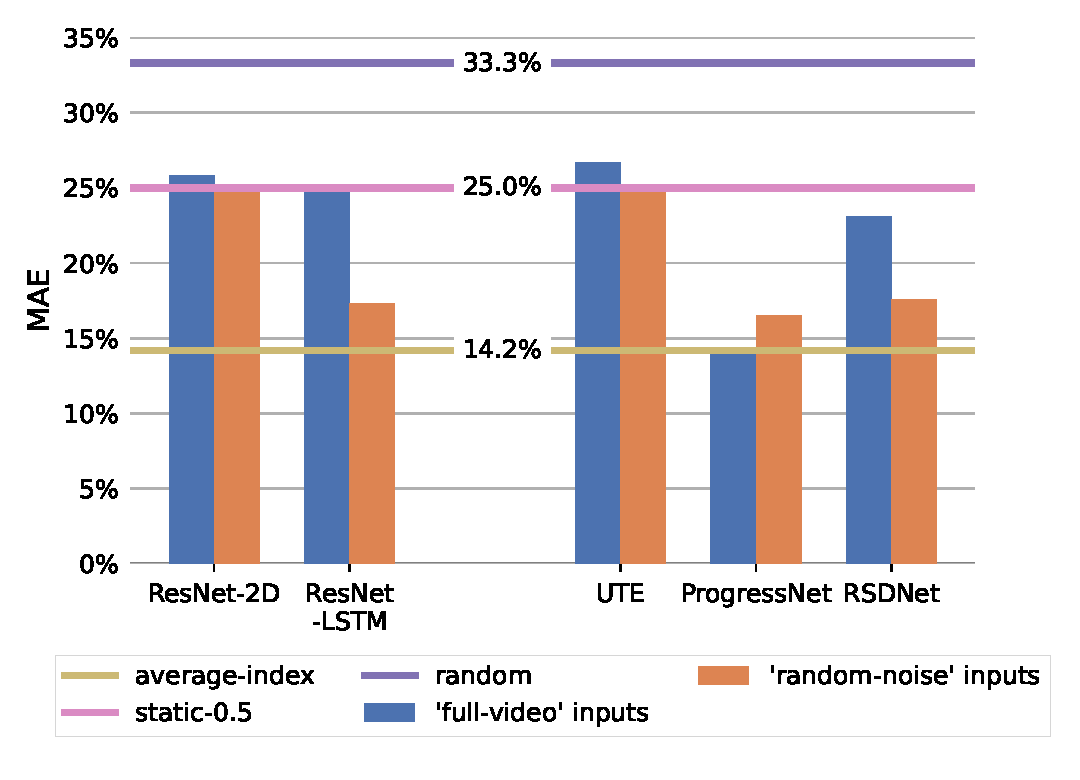
\includegraphics[width=1.0\linewidth]{iccv2023AuthorKit/media/results/UCF101-24_full_video_random.pdf}
\end{center}
   \caption{\textbf{UCF101-24 training on \textsl{full-videos}}. 
   MAE in percentages for all learning methods when inputting both \textsl{full-video} data and \textsl{random-noise}. 
   For all methods except \textsl{ProgressNet} inputting \textsl{random-noise} performs on par or better than inputting \textsl{full-videos}.
   % \slp{Please clarify in all legends that "full-videos" are input and "random-noise" as well: e.g. "`full-video' inputs". Now you have 2 random and that is confusing because one is a baseline and the other is an input. Also use "static-0.5", "'video-segment' inputs". Also not that I use "textsl" for all dataset names and method names and data settings.}
   }
\label{fig:result_ucf_seq}
\end{figure}
\begin{figure}
\begin{center}
   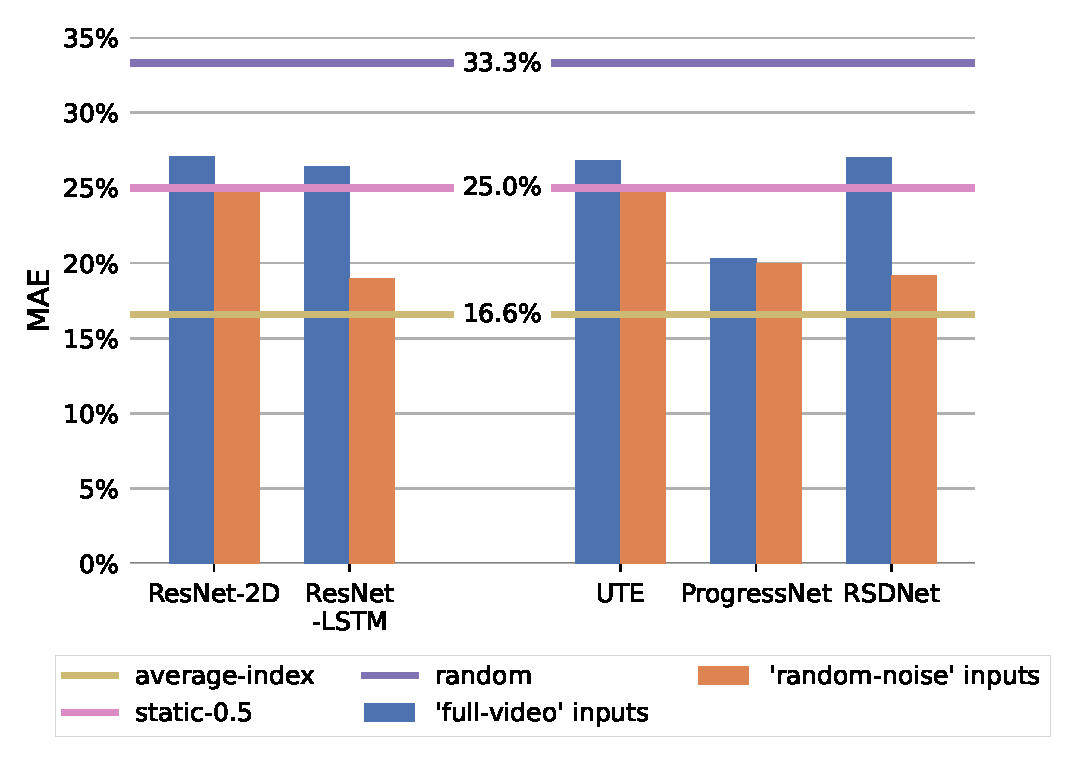
\includegraphics[width=1.0\linewidth]{iccv2023AuthorKit/media/results/Breakfast_full_video_random.pdf}
\end{center}
   \caption{\textbf{Breakfast training on \textsl{full-videos}}. 
   MAE in percentages for all learning methods when inputting \textsl{full-video} data and \textsl{random-noise}. 
   When using \textsl{random-noise} as input to the recurrent methods, they perform on par or better than when inputting \textsl{full-videos}, indicating that the methods learn to count video frames.}
\label{fig:result_breakfast_seq}
\end{figure}
\begin{figure}
\begin{center}
   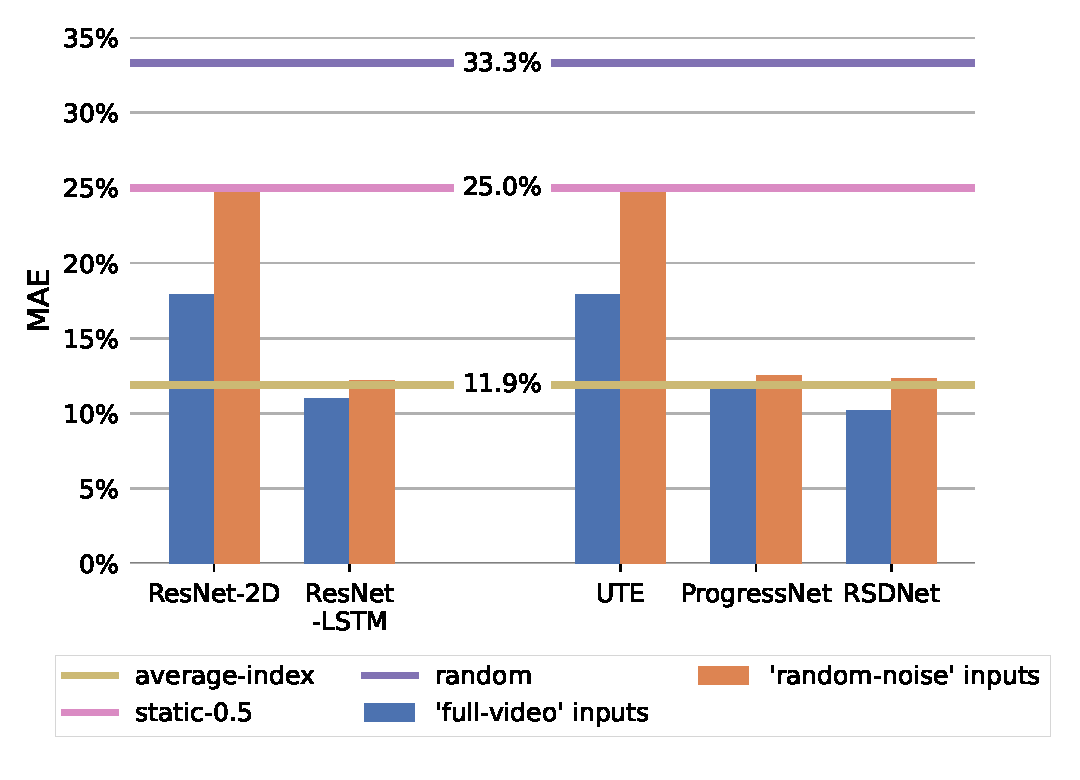
\includegraphics[width=1.0\linewidth]{iccv2023AuthorKit/media/results/Cholec80_full_video_random.pdf}
\end{center}
   \caption{\textbf{Cholec80 training on \textsl{full-videos}}. 
   MAE in percentages for all considered methods when inputting \textsl{full-videos} and \textsl{random-noise}. 
   On this dataset, all methods are able to learn from the visual data. 
   When provided with \textsl{random-noise}, the recurrent methods perform on par with the \textsl{average-index} baseline, estimating dataset statistics.}
\label{fig:result_cholec_seq}
\end{figure}

\fig{result_ucf_seq} shows that when training on \textsl{full-videos} of \textsl{UCF101-24} both the \textsl{ResNet-2D} model and \textsl{UTE} models perform on par with the \textsl{static-0.5} baseline.
This is because these spatial-only networks do not have any way of integrating temporal information and they fail to extract progress information from the visual data alone. 
When provided with \textsl{random-noise} as inputs, they always predict $0.5$ and score on par with the \textsl{static-0.5} baseline. 
The results are similar for the recurrent models, \textsl{ResNet-LSTM} and \textsl{RSDNet} who are both close to the \textsl{static-0.5} baseline. 
We observe that the recurrent models overfit on the embedded features and fail to generalise to the test set. 
When these recurrent networks are provided with \textsl{random-noise} they learn to count frames, and thus reach the \textsl{average-index} baseline. 
\textsl{ProgressNet} is the only outlier here: when given \textsl{full-video} data it performs better than the \textsl{average-index} baseline, and when given \textsl{random-noise} as inputs, it performs slightly worse. 
Since the visual information is not sufficiently informative to predict progress, as seen for the \textsl{ResNet-LSTM} and \textsl{RSDNet}, \textsl{ProgressNet} learns to count frames to aid in its progress predictions.

For \textsl{Breakfast} in \fig{result_breakfast_seq} the results look very similar to those on \textsl{UCF101-24}. 
Both the \textsl{ResNet-2D} and \textsl{UTE} models cannot learn from visual information alone. \textsl{ResNet-LSTM} and \textsl{RSDNet} both perform worse than the \textsl{static-0.5} baseline, indicating that they are overfitting on the training data. 
When provided with \textsl{random-noise} as input, they rely on frame counting. 
\textsl{ProgressNet} obtains similar results when given both \textsl{full-videos} and \textsl{random-noise}, indicating that in both cases it is performing frame counting.

\textsl{Cholec80} in \fig{result_cholec_seq} is the only dataset where the spatial-only networks \textsl{ResNet-2D} and \textsl{UTE} perform better than the \textsl{static-0.5} baseline.
This hints to the visual information present in this dataset being indicative of the activity progress. 
When inputting \textsl{random-noise} the methods again perform on par with the \textsl{static-0.5} baseline, as expected. 
Here, \textsl{ResNet-LSTM}, \textsl{RSDNet}, and \textsl{ProgressNet}, can make use of both the visual information and frame counting and perform slightly better than the \textsl{average-index} baseline. 
%When provided with \textsl{random-noise} inputs, these networks perform on par with the \textsl{average-index} baseline.
% these networks perform slightly worse, but still on par with the \textsl{average-index} \slp{Why are they better at counting here than on the other datasets?}. This may be due to the dataset length distribution not being skewed. 

\smallskip\noindent\textbf{Observation:} \emph{The progress prediction methods and the learning baselines can fail to extract useful information from video data. 
When this happens, memory-based methods will rely on frame counting when presented with \textsl{full-videos} as inputs.}

%-----------------------------------------------------------------------------------
\medskip\noindent\textbf{(i.2): Progress predictions on \textsl{video-segments}.}
We test what information learning methods use when trained to predict progress from \textsl{video-segments}.
Using \textsl{video-segments} should encourage the methods to focus more on the visual information and less so on the temporal position of the frames. 
We compare this with inputting \textsl{frame-indices} -- absolute frame indices replicated as images.
Ideally, we would expect all methods to solve the progress prediction task by relying on visual information, and therefore surpassing the scores obtained when inputting \textsl{frame-indices}.
Again, we also compare with the naive baselines: \textsl{static-0.5}, \textsl{random} and \textsl{average-index}. 

\begin{figure}
\begin{center}
   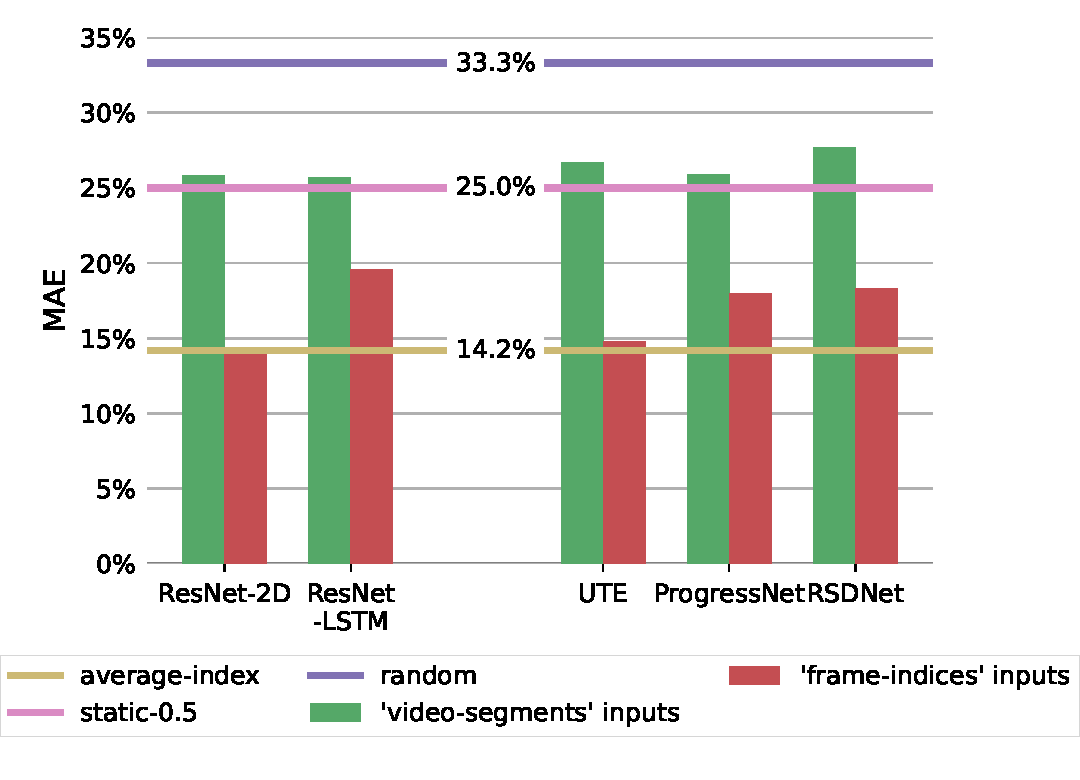
\includegraphics[width=1.0\linewidth]{iccv2023AuthorKit/media/results/UCF101-24_video_segments_indices.pdf}
\end{center}
   \caption{\textbf{
   \textsl{UCF101-24} training on \textsl{video-segments}}. 
   MAE in percentages for all considered methods when inputting both \textsl{video-segments} and \textsl{frame-indices}. 
   For all methods inputting \textsl{frame-indices} is better than inputting \textsl{video-segments}. 
   \textsl{ResNet-2D} and \textsl{UTE} get the biggest boost in performance because they can learn the one-to-one mapping from index to progress during training. 
   }
\label{fig:result_ucf_seg}
\end{figure}
\begin{figure}
\begin{center}
   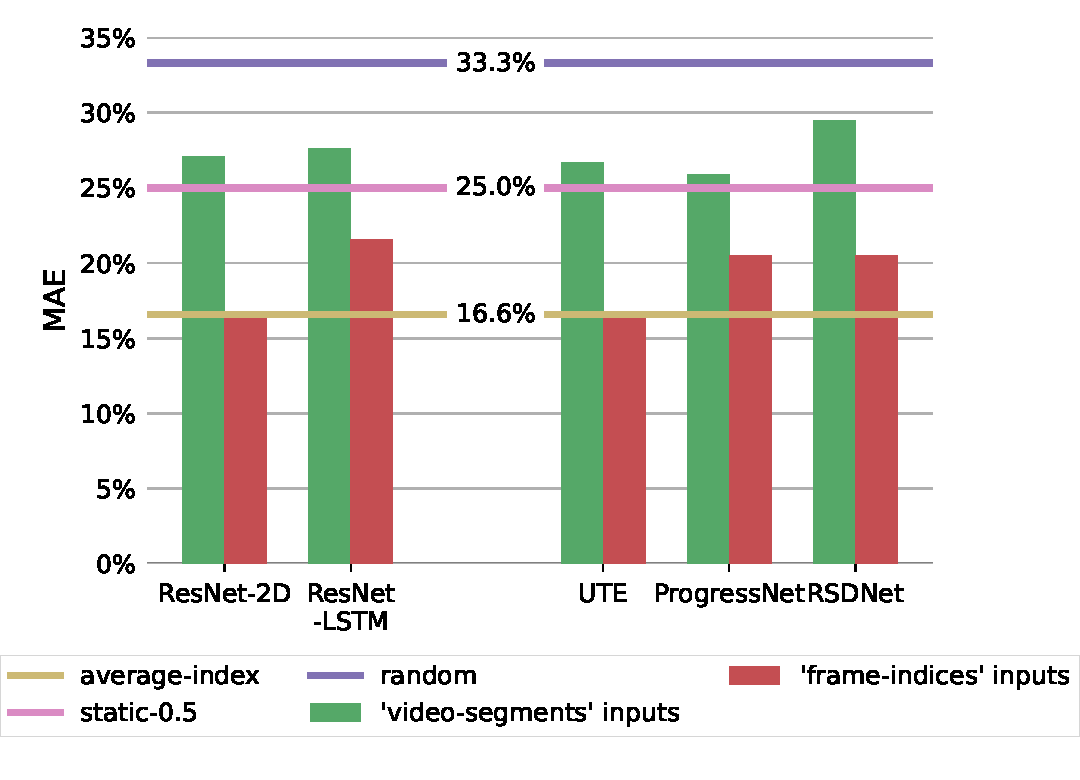
\includegraphics[width=1.0\linewidth]{iccv2023AuthorKit/media/results/Breakfast_video_segments_indices.pdf}
\end{center}
   \caption{\textbf{\textsl{Breakfast} training on \textsl{video-segments}}. 
   MAE in percentages for all considered methods when inputting both \textsl{video-segments} and \textsl{frame-indices}. 
   All methods perform better when using \textsl{frame-indices} as input. 
   Also here \textsl{ResNet-2D} and \textsl{UTE} obtain the lowest error.}
\label{fig:result_breakfast_seg}
\end{figure}
\begin{figure}
\begin{center}
   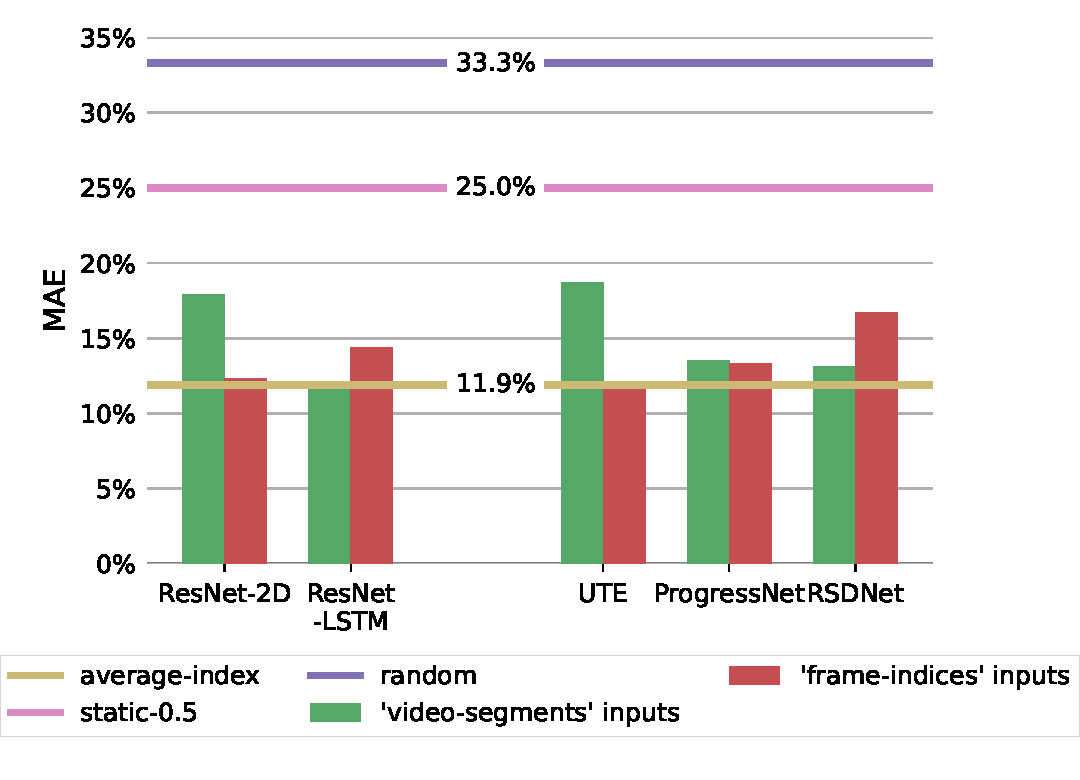
\includegraphics[width=1.0\linewidth]{iccv2023AuthorKit/media/results/Cholec80_video_segments_indices.pdf}
\end{center}
   \caption{\textbf{\textsl{Cholec80} training on \textsl{video-segments}}. 
   MAE in percentages for all considered methods when inputting both \textsl{video-segments} and \textsl{frame-indices}. 
   For \textsl{RSDNet} inputting \textsl{frame-indices} is slightly worse. 
   This could be due to suboptimal hyperparameter settings. 
   % Either the loss between the RSD and progress is not balanced, or the elapsed time features may be causing gradients that are too large.
   % This is because the RSD normalization factor $s_\text{norm}$, which balances the RSD and progress loss, is not optimal.
   }
\label{fig:result_cholec_seg}
\end{figure}

\fig{result_ucf_seg} shows that when trained on \textsl{video-segments} of \textsl{UCF101-24} all methods perform on par with the \textsl{static-0.5} baseline.
Thus, the models cannot learn to predict progress from the visual video data. 
Interestingly, \textsl{ProgressNet} using \textsl{full-videos} in \fig{result_ucf_seq} is better than the \textsl{average-index} baseline, however, here it fails to learn when trained on \textsl{video-segments}. 
This suggests that on the \textsl{full-videos} the network was not relying on the visual information, but just on the temporal progression of frames -- frame counts. 
When provided with \textsl{frame-indices} as input, all methods improve. 
The improvement is most visible for \textsl{ResNet-2D} and \textsl{UTE}, which do not use recurrent blocks. 
This is because the non-recurrent methods can learn the one-to-one mapping from index to progress during training and apply it at test-time. 
%Recurrent methods must learn this mapping in a sequence, which differs between training and testing.
% \slp{Give a sentence here why does these 2 improve the most?}

The results on \textsl{Breakfast} in \fig{result_breakfast_seg} are similar to those of \textsl{UCF101-24} in \fig{result_ucf_seg}. 
None of the networks can extract useful information from the \textsl{video-segments}.
And, as expected, \textsl{ProgressNet} performs worse than when trained on \textsl{full-videos}. 
All methods improve when trained on \textsl{frame-indices}.
The improvement is again more obvious for \textsl{ResNet-2D} and \textsl{UTE}.

On \textsl{Cholec80} in \fig{result_cholec_seg} we see a similar trend. 
\textsl{ResNet-2D} and \textsl{UTE} improve when provided with \textsl{frame-indices} as input. 
For \textsl{ResNet-LSTM} and \textsl{ProgressNet} the performance is on par with the \textsl{average-index} baseline for both \textsl{video-sequences} and \textsl{frame-indices} as inputs, indicating that on the \textsl{Cholec80} these methods can learn progress prediction from visual information, however, they still cannot perform better than the \textsl{average-index} baseline. 
\textsl{RSDNet} performs worst when given \textsl{frame-indices} as inputs;  we hypothesise that this is due suboptimal hyperparameter settings. 
%Either the loss between the RSD and progress is not balanced, or the elapsed time features may be causing gradients that are too large.
% to the joint optimization of progress and RSD. 
% \textsl{RSDNet} uses an RSD normalization factor $s_\text{norm}$ to balance out the loss between the RSD head and the progress head. 
% The results on \textsl{RSDNet} may be due to us not having found an optimal value for this normalization factor.

\smallskip\noindent\textbf{Observation:} \emph{The progress prediction methods cannot extract sufficient information from visual data for solving the progress prediction, on the currently used datasets. And when not provided with the complete videos, these methods are outperformed by native non-learning baselines relying on data statistics.}


%-------------------------------------------------------------------------------
\subsection{\emph{\textbf{(ii) Is it at all possible to predict activity progress from visual data only?}}}
We observe that existing learning-based methods often fail to extract progress information from visual data alone. 
Our goal here is to construct a synthetic dataset in such a way that the learning-based methods perform optimal using visual information, and outperform the naive baselines.

We construct a synthetic \textsl{Progress-bar} dataset, as shown in \fig{progressbars}. 
The dataset contains a progress bar (similar, for example, to a download bar) that slowly fills up from left to right. 
Each frame has a resolution of $32{\times}32$px. 
We generate $900$ videos for the training split, and $100$ for the test split.
% \slp{should you also not generate a val split for hyper-parameter setting?}
Each bar has its own rate of progression, but there is a variance per notch causing some uncertainty. 
This is why in the first image the progression appears to be slightly beyond 25\%, but because the video may slow down after this section it is actually at 22.2\%. 
Due to the large variance in video length, ranging from $19$ to $145$ frames, the \textsl{average-index} baseline, and thus frame-counting strategies, will give worse results than relying on visual information.
Also, because of the different progress rates per video, the learning methods cannot just rely on visual information alone but also have to use memory to perform well on this progress prediction task. 
% \slp{Add some more info about the dataset: what is the frame resolution: 64x64px? How many videos did you create, how many you have for train/val/test?}
%\slp{Can you add here a few sentences on how the methods have changed:i.e. Because of the dataset size and reduced complexity, we scale down the backbones of all the learning models. Specifically we use ResNet-18 for ... bla bla , and ..}


\begin{figure}[t]
\begin{center}
   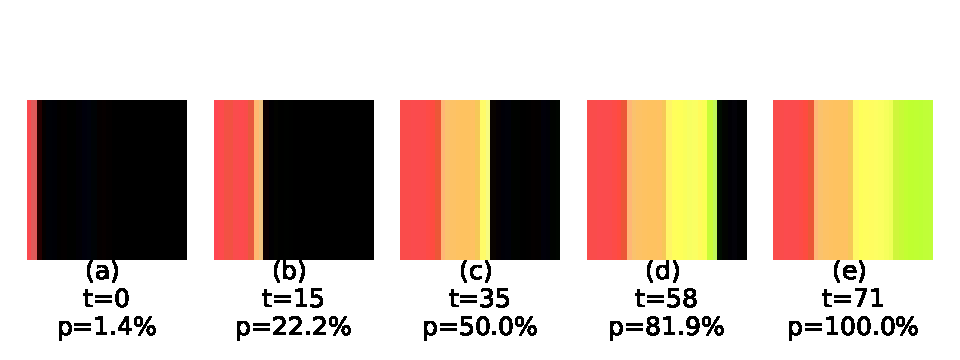
\includegraphics[width=1.0\linewidth]{iccv2023AuthorKit/media/bars.pdf}
\end{center}
   \caption{Visualisation of a progress bar from our synthetic \textsl{Progress-bar} dataset at timesteps $t{=}0$, $t{=}15$, $t{=}35$, $t{=}58$, and $t{=}71$. 
   Each coloured section indicates visually a 25\% section, but due to variance in the speed, the actual video progress may differ at these points.
   }
\label{fig:progressbars}
\end{figure}
Due to the reduced frame resolution and data complexity of our synthetic dataset, we scale down the \textsl{ResNet} backbone, for these experiments. 
Specifically, to avoid overfitting, we use \textsl{ResNet-18} as a backbone for \textsl{ResNet-2D}, \textsl{ResNet-LSTM}, and \textsl{RSDNet}. 
\textsl{ProgressNet} and \textsl{UTE} remain unchanged.


\fig{result_bars} shows the results of all the learning-based methods when predicting progress from both \textsl{full-videos} and \textsl{video-segments}. 
For this dataset the \textsl{average-index} baseline has an MAE of $12.9$\%, which is outperformed by all learning-based methods. 
\textsl{UTE} performs the best out of all the networks, even though it does not have memory. 
This is because \textsl{UTE} uses frame embeddings with a temporal-window size of $16$ frames. 
This temporal-window gives the method information about $7$ future frames, which is sufficient on this simple dataset. 
For the LSTM-based methods inputting \textsl{full-videos} still performs slightly better than inputting \textsl{video-segments}. 
At a closer look, this is because the \textsl{video-segments} sampling method has a bias towards frames in the middle of a video. 
The earlier frames are less likely to get sampled, thus the progress prediction methods will have a higher error here.
% \slp{Say why is this happening}

\smallskip\noindent\textbf{Observation:} \emph{It is feasible for the progress prediction methods to make effective use of the visual data present in the videos and outperform the \textsl{average-index} baseline, when the visual data is a clear indicator of the video progression.
}
\begin{figure}
\begin{center}
   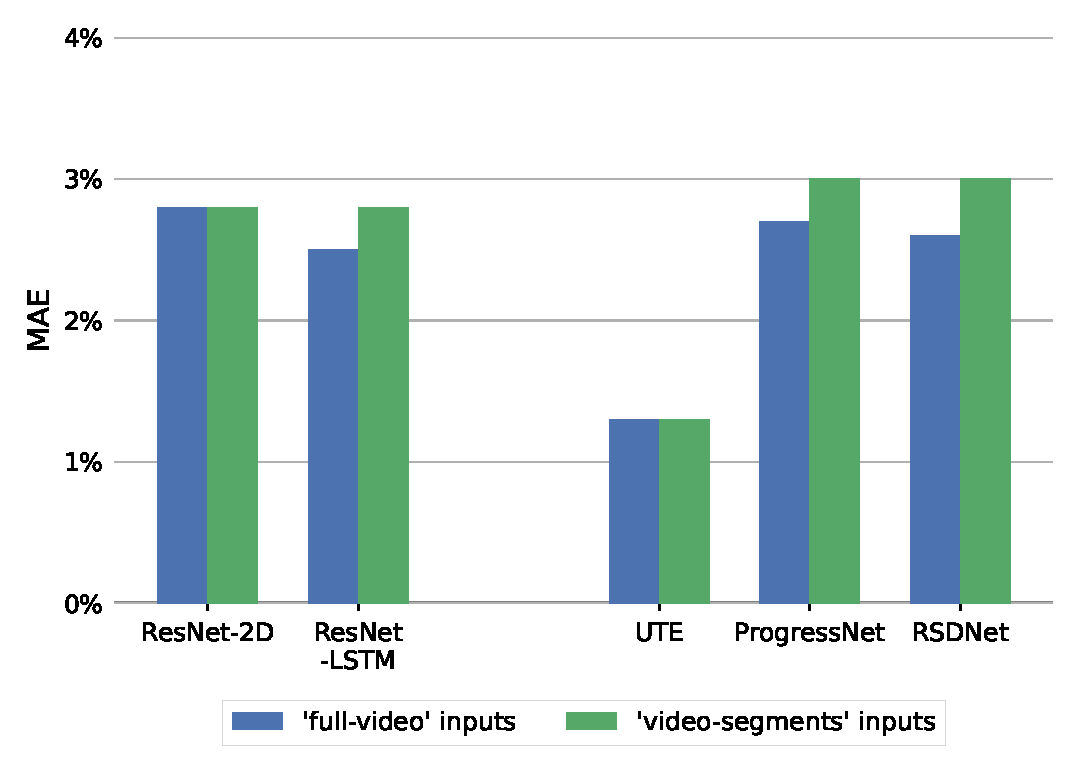
\includegraphics[width=1.0\linewidth]{iccv2023AuthorKit/media/results/Bars_full_video_video_segments.pdf}
\end{center}
   \caption{\textbf{MAE scores on our synthetic \textsl{Progress-bar} dataset, when training on \textsl{full-videos} and \textsl{video-segments}}. 
   The \textsl{average-index} baseline has an MAE of $12.9\%$, while the \textsl{static} baseline is at $25\%$ and the \textsl{random} baseline at $33.3\%$. 
   We see that all methods outperform the \textsl{average-index} baseline. 
   \textsl{UTE} obtains the best result due to its $15$-frame temporal window, which allows it to see $7$ frames into the future. 
   We conclude that the progress prediction methods are able to learn progress from visual information, if it is clearly present in the videos.}
\label{fig:result_bars}
\end{figure}